
% LaTeX-Vorlage für Versuchsprotokolle
% Autor: Simon May
% Datum: 2017-10-05

% Es gibt die Dokumenttypen scrartcl („Artikel“), scrreprt („Bericht“),
% scrbook („Buch“) und scrlttr2 („Brief“). Diese gehören zum KOMA-Script,
% bieten mehr Optionen als die „Standardklassen“ und sollten besonders für
% deutsche Texte benutzt werden.
% Natürlich gibt es noch weitere Klassen, z.B. beamer für Präsentationen.
\documentclass[
	a4paper,                % Papierformat (DIN A4)
	titlepage=firstiscover, % Separate Titelseite
	captions=tableheading,  % \caption bei Tabellen immer als Überschrift setzen
	toc=bibliography,       % Literaturverzeichnis im Inhaltsverzeichnis aufführen
	toc=listof,             % Abbildungsverzeichnis etc. im Inhaltsverzeichnis aufführen
	oneside,                % Einseitig
	%twoside,               % Zweiseitig
	%twocolumn,             % Zweispaltig
	automark,               % Abschnittstitel automatisch in Kopfzeile einfügen
	12pt,                   % Schriftgröße (beliebige Größen mit „fontsize=Xpt“)
	english, ngerman,       % Sprache für z.B. Babel; ausgewählt: ngerman (letztgenannt)
	%draft=true             % Entwurf-Modus; markiert zu lange und zu kurze Zeilen
]{scrartcl}

% --- Pakete einbinden
% Autor: Simon May
% Datum: 2017-10-04

% --- Pakete einbinden
% --- Pakete erweitern LaTeX um zusätzliche Funktionen.
%     Dies ist ein Satz nützlicher Pakete.

% Silbentrennung etc.; Sprache wird durch Option bei \documentclass festgelegt
\usepackage{babel}
\usepackage{iftex}
\ifLuaTeX
	% Schriftart (Latin Modern)
	\usepackage{fontspec}
	\fontspec{Latin Modern Roman}
\else
	% Verwendung der Zeichentabelle T1 (für Sonderzeichen etc.)
	\usepackage[T1]{fontenc}
	% Legt die Eingabe-Zeichenkodierung fest, z.B. UTF-8
	\usepackage[utf8]{inputenc}
	% Schriftart (Latin Modern)
	\usepackage{lmodern}
	% Zusätzliche Sonderzeichen
	\usepackage{textcomp}
\fi

% Nutzen von +, -, *, / in \setlength u.ä. (z.B. \setlength{\a + 3cm})
\usepackage{calc}
% Wird benötigt, um \ifthenelse zu benutzen
\usepackage{xifthen}
% Optionen für eigene definierte Befehle
\usepackage{xparse}

% Verbessertes Aussehen des Schriftbilds durch kleine Anpassungen
\usepackage{microtype}
% Automatische Formatierung von Daten
\usepackage[useregional]{datetime2}
% Wird für Kopf- und Fußzeile benötigt
\usepackage{scrlayer-scrpage}
% Einfaches Wechseln zwischen unterschiedlichen Zeilenabständen
\usepackage{setspace}
% Optionen für Listen (enumerate, itemize, …)
\usepackage{enumitem}
% Automatische Anführungszeichen
\usepackage{csquotes}
% Zusätzliche Optionen für Tabellen (tabular)
\usepackage{array}

% Mathepaket (intlimits: Grenzen über/unter Integralzeichen)
\usepackage[intlimits]{amsmath}
% Mathe-Symbole, \mathbb etc.
\usepackage{amssymb}
% Weitere Mathebefehle
\usepackage{mathtools}
% „Schöne“ Brüche im Fließtext
\usepackage{xfrac}
% Ermöglicht die Nutzung von \SI{Zahl}{Einheit} u.a.
\usepackage{siunitx}
% Definition von Unicode-Symbolen; Nach [utf8]inputenc laden!
\usepackage{newunicodechar}
% Unicode-Formeln mit pdfLaTeX
% Autor: Simon May
% Datum: 2015-03-04

% Diese Datei ermöglicht es, Mathe-Symbole (z.B. \gamma) direkt als
% Sonderzeichen (d.h. γ) einzugeben

% silence unterdrückt Warnungen; vor hyperref laden
\usepackage{silence}
\WarningFilter[pdflatex-unicode-math]{newunicodechar}{Redefining Unicode character}
\ActivateWarningFilters[pdflatex-unicode-math]

\newunicodechar{†}{\dag}
\newunicodechar{‡}{\ddag}
\newunicodechar{…}{\ldots}
\newunicodechar{⋯}{\cdots}
\newunicodechar{⋮}{\vdots}
\newunicodechar{⋱}{\ddots}
\newunicodechar{⋰}{\iddots}
\newunicodechar{α}{\alpha}
\newunicodechar{β}{\beta}
\newunicodechar{γ}{\gamma}
\newunicodechar{δ}{\delta}
\newunicodechar{ε}{\varepsilon}
\newunicodechar{ϵ}{\epsilon}
\newunicodechar{ζ}{\zeta}
\newunicodechar{η}{\eta}
\newunicodechar{θ}{\theta}
\newunicodechar{ϑ}{\vartheta}
\newunicodechar{ι}{\iota}
\newunicodechar{κ}{\kappa}
\newunicodechar{ϰ}{\varkappa}
\newunicodechar{λ}{\lambda}
\newunicodechar{μ}{\mu}
\newunicodechar{ν}{\nu}
\newunicodechar{ξ}{\xi}
\newunicodechar{ο}{o}
\newunicodechar{π}{\pi}
\newunicodechar{ρ}{\rho}
\newunicodechar{ϱ}{\varrho}
\newunicodechar{σ}{\sigma}
\newunicodechar{τ}{\tau}
\newunicodechar{υ}{\upsilon}
\newunicodechar{φ}{\varphi}
\newunicodechar{ϕ}{\phi}
\newunicodechar{χ}{\chi}
\newunicodechar{ψ}{\psi}
\newunicodechar{ω}{\omega}
\newunicodechar{Α}{\mathrm{A}}
\newunicodechar{Β}{\mathrm{B}}
\newunicodechar{Γ}{\Gamma}
\newunicodechar{Δ}{\Delta}
\newunicodechar{Ε}{\mathrm{E}}
\newunicodechar{Ζ}{\mathrm{Z}}
\newunicodechar{Η}{\mathrm{H}}
\newunicodechar{Θ}{\Theta}
\newunicodechar{Ι}{\mathrm{I}}
\newunicodechar{Κ}{\mathrm{K}}
\newunicodechar{Λ}{\Lambda}
\newunicodechar{Μ}{\mathrm{M}}
\newunicodechar{Ν}{\mathrm{N}}
\newunicodechar{Ξ}{\Xi}
\newunicodechar{Ο}{\mathrm{O}}
\newunicodechar{Π}{\Pi}
\newunicodechar{Ρ}{\mathrm{P}}
\newunicodechar{Σ}{\Sigma}
\newunicodechar{Τ}{\mathrm{T}}
\newunicodechar{Υ}{\Upsilon}
\newunicodechar{Φ}{\Phi}
\newunicodechar{Χ}{\Chi}
\newunicodechar{Ψ}{\Psi}
\newunicodechar{Ω}{\Omega}
\newunicodechar{∑}{\sum}
\newunicodechar{∫}{\int}
\newunicodechar{∬}{\iint}
\newunicodechar{∭}{\iiint}
\newunicodechar{⨌}{\iiiint}
\newunicodechar{∮}{\oint}
\newunicodechar{∯}{\oiint}
\newunicodechar{∰}{\oiiint}
\newunicodechar{∇}{\nabla}
\newunicodechar{∂}{\partial}
\newunicodechar{√}{\sqrt}
\newunicodechar{∈}{\in}
\newunicodechar{∋}{\ni}
\newunicodechar{∉}{\notin}
\newunicodechar{∀}{\forall}
\newunicodechar{∃}{\exists}
\newunicodechar{∄}{\nexists}
\newunicodechar{∴}{\therefore}
\newunicodechar{∵}{\because}
\newunicodechar{〈}{\langle}
\newunicodechar{〉}{\rangle}
\newunicodechar{⌊}{\lfloor}
\newunicodechar{⌋}{\rfloor}
\newunicodechar{⌈}{\lceil}
\newunicodechar{⌉}{\rceil}
\newunicodechar{∼}{\sim}
\newunicodechar{∝}{\propto}
\newunicodechar{∞}{\infty}
\newunicodechar{ℵ}{\aleph}
\newunicodechar{ℏ}{\hbar}
\newunicodechar{℘}{\wp}
\newunicodechar{ℓ}{\ell}
\newunicodechar{∅}{\emptyset}
\newunicodechar{×}{\times}
\newunicodechar{⋅}{\cdot}
\newunicodechar{÷}{\div}
\newunicodechar{⋆}{\star}
\newunicodechar{∘}{\circ}
\newunicodechar{⋄}{\diamond}
\newunicodechar{⊕}{\oplus}
\newunicodechar{⊖}{\ominus}
\newunicodechar{⊗}{\otimes}
\newunicodechar{⊘}{\oslash}
\newunicodechar{⊙}{\odot}
\newunicodechar{±}{\pm}
\newunicodechar{∓}{\mp}
\newunicodechar{≈}{\approx}
\newunicodechar{≡}{\equiv}
\newunicodechar{≠}{\ne}
\newunicodechar{≥}{\ge}
\newunicodechar{≤}{\le}
\newunicodechar{≫}{\gg}
\newunicodechar{≪}{\ll}
\newunicodechar{⊂}{\subset}
\newunicodechar{⊃}{\supset}
\newunicodechar{⊆}{\subseteq}
\newunicodechar{⊇}{\supseteq}
\newunicodechar{⊈}{\nsubseteq}
\newunicodechar{⊉}{\nsupseteq}
\newunicodechar{≔}{\coloneqq}
\newunicodechar{≕}{\eqqcolon}
\newunicodechar{¬}{\neg}
\newunicodechar{∨}{\vee}
\newunicodechar{∧}{\wedge}
\newunicodechar{∪}{\cup}
\newunicodechar{∩}{\cap}
\newunicodechar{⋁}{\bigvee}
\newunicodechar{⋀}{\bigwedge}
\newunicodechar{⋃}{\bigcup}
\newunicodechar{⋂}{\bigcap}
\newunicodechar{⟂}{\perp}
\newunicodechar{∥}{\parallel}
\newunicodechar{∦}{\nparallel}
\newunicodechar{𝚤}{\imath}
\newunicodechar{𝚥}{\jmath}
\newunicodechar{⇔}{\Leftrightarrow}
\newunicodechar{⇕}{\Updownarrow}
\newunicodechar{⇐}{\Leftarrow}
\newunicodechar{⇒}{\Rightarrow}
\newunicodechar{⇑}{\Uparrow}
\newunicodechar{⇓}{\Downarrow}
\newunicodechar{↔}{\leftrightarrow}
\newunicodechar{↕}{\updownarrow}
\newunicodechar{←}{\leftarrow}
\newunicodechar{→}{\rightarrow}
\newunicodechar{↑}{\uparrow}
\newunicodechar{↓}{\downarrow}
\newunicodechar{⟷}{\longleftrightarrow}
\newunicodechar{⟵}{\longleftarrow}
\newunicodechar{⟶}{\longrightarrow}
\newunicodechar{⇇}{\leftleftarrows}
\newunicodechar{⇉}{\rightrightarrows}
\newunicodechar{⇈}{\upuparrows}
\newunicodechar{⇊}{\downdownarrows}
\newunicodechar{⟺}{\Longleftrightarrow}
\newunicodechar{⟸}{\Longleftarrow}
\newunicodechar{⟹}{\Longrightarrow}
\newunicodechar{↦}{\mapsto}
\newunicodechar{↤}{\mapsfrom}
\newunicodechar{⟼}{\longmapsto}
\newunicodechar{⟻}{\longmapsfrom}
\newunicodechar{⟾}{\Longmapsto}
\newunicodechar{⟽}{\Longmapsfrom}
\newunicodechar{↗}{\nearrow}
\newunicodechar{↖}{\nwarrow}
\newunicodechar{↘}{\searrow}
\newunicodechar{↙}{\swarrow}
\newunicodechar{↩}{\hookleftarrow}
\newunicodechar{↪}{\hookrightarrow}
\newunicodechar{↶}{\curvearrowleft}
\newunicodechar{↷}{\curvearrowright}
\newunicodechar{↺}{\circlearrowleft}
\newunicodechar{↻}{\circlearrowright}
\newunicodechar{↫}{\looparrowleft}
\newunicodechar{↬}{\looparrowright}
\newunicodechar{⇋}{\leftrightharpoons}
\newunicodechar{⇌}{\rightleftharpoons}
\newunicodechar{↼}{\leftharpoonup}
\newunicodechar{↽}{\leftharpoondown}
\newunicodechar{⇀}{\rightharpoonup}
\newunicodechar{⇁}{\rightharpoondown}
\newunicodechar{↿}{\upharpoonleft}
\newunicodechar{↾}{\upharpoonright}
\newunicodechar{⇃}{\downharpoonleft}
\newunicodechar{⇂}{\downharpoonright}
\newunicodechar{𝔸}{\mathbb{A}}
\newunicodechar{𝔹}{\mathbb{B}}
\newunicodechar{ℂ}{\mathbb{C}}
\newunicodechar{𝔻}{\mathbb{D}}
\newunicodechar{𝔼}{\mathbb{E}}
\newunicodechar{𝔽}{\mathbb{F}}
\newunicodechar{𝔾}{\mathbb{G}}
\newunicodechar{ℍ}{\mathbb{H}}
\newunicodechar{𝕀}{\mathbb{I}}
\newunicodechar{𝕁}{\mathbb{J}}
\newunicodechar{𝕂}{\mathbb{K}}
\newunicodechar{𝕃}{\mathbb{L}}
\newunicodechar{𝕄}{\mathbb{M}}
\newunicodechar{ℕ}{\mathbb{N}}
\newunicodechar{𝕆}{\mathbb{O}}
\newunicodechar{ℙ}{\mathbb{P}}
\newunicodechar{ℚ}{\mathbb{Q}}
\newunicodechar{ℝ}{\mathbb{R}}
\newunicodechar{𝕊}{\mathbb{S}}
\newunicodechar{𝕋}{\mathbb{T}}
\newunicodechar{𝕌}{\mathbb{U}}
\newunicodechar{𝕍}{\mathbb{V}}
\newunicodechar{𝕎}{\mathbb{W}}
\newunicodechar{𝕏}{\mathbb{X}}
\newunicodechar{𝕐}{\mathbb{Y}}
\newunicodechar{ℤ}{\mathbb{Z}}
\newunicodechar{𝒜}{\mathcal{A}}
\newunicodechar{ℬ}{\mathcal{B}}
\newunicodechar{𝒞}{\mathcal{C}}
\newunicodechar{𝒟}{\mathcal{D}}
\newunicodechar{ℰ}{\mathcal{E}}
\newunicodechar{ℱ}{\mathcal{F}}
\newunicodechar{𝒢}{\mathcal{G}}
\newunicodechar{ℋ}{\mathcal{H}}
\newunicodechar{ℐ}{\mathcal{I}}
\newunicodechar{𝒥}{\mathcal{J}}
\newunicodechar{𝒦}{\mathcal{K}}
\newunicodechar{ℒ}{\mathcal{L}}
\newunicodechar{ℳ}{\mathcal{M}}
\newunicodechar{𝒩}{\mathcal{N}}
\newunicodechar{𝒪}{\mathcal{O}}
\newunicodechar{𝒫}{\mathcal{P}}
\newunicodechar{𝒬}{\mathcal{Q}}
\newunicodechar{ℛ}{\mathcal{R}}
\newunicodechar{𝒮}{\mathcal{S}}
\newunicodechar{𝒯}{\mathcal{T}}
\newunicodechar{𝒰}{\mathcal{U}}
\newunicodechar{𝒱}{\mathcal{V}}
\newunicodechar{𝒲}{\mathcal{W}}
\newunicodechar{𝒳}{\mathcal{X}}
\newunicodechar{𝒴}{\mathcal{Y}}
\newunicodechar{𝒵}{\mathcal{Z}}
\newunicodechar{𝕬}{\mathfrak{A}}
\newunicodechar{𝕭}{\mathfrak{B}}
\newunicodechar{𝕮}{\mathfrak{C}}
\newunicodechar{𝕯}{\mathfrak{D}}
\newunicodechar{𝕰}{\mathfrak{E}}
\newunicodechar{𝕱}{\mathfrak{F}}
\newunicodechar{𝕲}{\mathfrak{G}}
\newunicodechar{𝕳}{\mathfrak{H}}
\newunicodechar{𝕴}{\mathfrak{I}}
\newunicodechar{𝕵}{\mathfrak{J}}
\newunicodechar{𝕶}{\mathfrak{K}}
\newunicodechar{𝕷}{\mathfrak{L}}
\newunicodechar{𝕸}{\mathfrak{M}}
\newunicodechar{𝕹}{\mathfrak{N}}
\newunicodechar{𝕺}{\mathfrak{O}}
\newunicodechar{𝕻}{\mathfrak{P}}
\newunicodechar{𝕼}{\mathfrak{Q}}
\newunicodechar{𝕽}{\mathfrak{R}}
\newunicodechar{𝕾}{\mathfrak{S}}
\newunicodechar{𝕿}{\mathfrak{T}}
\newunicodechar{𝖀}{\mathfrak{U}}
\newunicodechar{𝖁}{\mathfrak{V}}
\newunicodechar{𝖂}{\mathfrak{W}}
\newunicodechar{𝖃}{\mathfrak{X}}
\newunicodechar{𝖄}{\mathfrak{Y}}
\newunicodechar{𝖅}{\mathfrak{Z}}

\DeactivateWarningFilters[pdflatex-unicode-math]


% Farben
\usepackage{xcolor}
% Einbinden von Grafiken (\includegraphics)
\usepackage{graphicx}
% .tex-Dateien mit \includegraphics einbinden
\usepackage{gincltex}
% Größere Freiheiten bei Dateinamen mit \includegraphics
\usepackage{grffile}
% Abbildungen im Fließtext
\usepackage{wrapfig}
% Zitieren, Bibliographie (Biber als Bibliographie-Programm verwenden!)
\usepackage[style=verbose, backend=biber]{biblatex}
% Abbildungen nebeneinander (subfigure, subtable)
\usepackage{subcaption}

% Verlinkt Textstellen im PDF-Dokument (sollte am Ende geladen werden)
\usepackage[unicode]{hyperref}
% „Schlaue“ Referenzen (nach hyperref laden!)
\usepackage{cleveref}
%PDF einbinden
%\usepackage{pdfpages}
%Graphiken zeichnen
%\usepackage{tikz}
%\usetikzlibrary{angles,quotes,babel,3d}
% --- Einstellungen
% -- LaTeX/KOMA
% 1,5-facher Zeilenabstand
\onehalfspacing
\recalctypearea
% Schrift bei Bildunterschriften ändern
\addtokomafont{caption}{\small}
\addtokomafont{captionlabel}{\bfseries}
% Nummerierung der Formeln entsprechend des Abschnitts (z.B. 1.1)
\numberwithin{equation}{section}
% „Verwaiste“ Zeilen am Seitenanfang/-Ende stärker vermeiden
\clubpenalty=1000
\widowpenalty=1000
% Auf mehrere Seiten aufgespaltene Fußnoten stärker vermeiden
\interfootnotelinepenalty=3000

% -- csquotes
% Anführungszeichen automatisch umwandeln
\MakeOuterQuote{"}

% -- siunitx
\sisetup{
	locale=DE,
	separate-uncertainty,
	output-product=\cdot,
	quotient-mode=fraction,
	per-mode=fraction,
	fraction-function=\sfrac
}

% -- hyperref
\hypersetup{
	% Links/Verweise mit Kasten der Dicke 0.5pt versehen
	pdfborder={0 0 0.5}
}

% -- cleveref
\crefname{equation}{}{}
\Crefname{equation}{}{}

% -- biblatex (Literaturverzeichnis)
\IfFileExists{res/literatur.bib}{
	\addbibresource{res/literatur.bib}
}{}

\AtEndPreamble{
	% Kopf- und Fußzeile konfigurieren
	\ifthenelse{\boolean{showHeader}}{
		\KOMAoptions{headsepline}
		\recalctypearea
		\automark{section}
		% Innenseite der Kopfzeile
		\ihead{\headmark}
		% Mitte der Kopfzeile
		\chead{}
		% Außenseite der Kopfzeile
		\ohead{\usekomafont{pagehead}\varAutor}
	}{}
	% Innnenseite der Fußzeile
	\ifoot{}
	% Mitte der Fußzeile          
	\cfoot{-~\pagemark~-}
	% Außenseite der Fußzeile
	\ofoot{}

	% Metadaten für die PDF-Datei
	\hypersetup{
		pdftitle={Versuchsprotokoll: \varName},
		pdfauthor={\varAutor},
		pdfsubject={Grundpraktikum},
		pdfkeywords={Physik, Münster, Praktikum, Versuchsprotokoll}
	}
}



% --- Eigene Befehle einbinden
% Autor: Simon May
% Datum: 2017-10-05

% Eigene Befehle eignen sich gut, um Abkürzungen für lange Befehle zu erstellen.
% So vermeidet man, dass man immer wieder dasselbe Konstrukt kopieren und
% einfügen muss und, wenn man dann doch etwas ändern will, an zahllosen Stellen
% im Dokument dieselbe Änderung vornehmen muss.
% Die Syntax ist die folgende:
% \newcommand{neuer Befahl}[Anzahl Parameter (optional)]{Inhalt}
% Das folgende Beispiel fügt ein Bild mit bestimmten vorgegebenen Optionen ein:
\newcommand{\centeredImage}[1]{
	\begin{figure}
		\centering
		\includegraphics[width=0.5\textwidth]{#1}
	\end{figure}
}
% #1 ist dabei ein Parameter, den man \centeredImage übergeben muss, also:
% \centeredImage{...}
% Benötigt man keine Parameter, dann lässt man [1] weg. Werden zusätzliche
% Parameter benötigt, dann kann man die Zahl auf maximal 9 erhöhen.

% Ein Befehl, um eine E-Mail-Adresse darzustellen bzw. automatisch zu verlinken
\newcommand{\email}[1]{\href{mailto:#1}{\texttt{#1}}}

% \arsinh etc.
\newcommand*{\arsinh}{\operatorname{arsinh}}
\newcommand*{\arcosh}{\operatorname{arcosh}}
\newcommand*{\artanh}{\operatorname{artanh}}
\newcommand*{\const}{\text{const.}}


% --- Variablen importieren
% Autor: Simon May
% Datum: 2016-10-13
% Der Befehl \newcommand kann auch benutzt werden, um „Variablen“ zu definieren:

% Nummer laut Praktikumsheft:
\newcommand*{\varNum}{M3}
% Name laut Praktikumsheft:
\newcommand*{\varName}{Elastizität}
% Datum der Durchführung (Format: JJJJ-MM-TT):
\newcommand*{\varDatum}{2017-12-00}
% Autoren des Protokolls:
\newcommand*{\varAutor}{Hauke Hawighorst, Jörn Sieveneck}
% Nummer der eigenen Gruppe:
\newcommand*{\varGruppe}{Gruppe 9}
% E-Mail-Adressen der Autoren (kommagetrennt ohne Leerzeichen!):
\newcommand{\varEmail}{h.hawighorst@uni-muenster.de,j\_siev11@uni-muenster.de}
%betreuer Name
\newcommand{\varBetreuer}{\normalsize betreut von \\ Christian Thiede  }
% E-Mail-Adresse anzeigen (true/false):
\newcommand*{\varZeigeEmail}{true}
% Kopfzeile anzeigen (true/false):
\newcommand*{\varZeigeKopfzeile}{true}
% Inhaltsverzeichnis anzeigen (true/false):
\newcommand*{\varZeigeInhaltsverzeichnis}{true}
% Literaturverzeichnis anzeigen (true/false):
\newcommand*{\varZeigeLiteraturverzeichnis}{true}


\newboolean{showEmail}
\setboolean{showEmail}{\varZeigeEmail}
\newboolean{showHeader}
\setboolean{showHeader}{\varZeigeKopfzeile}
\newboolean{showTOC}
\setboolean{showTOC}{\varZeigeInhaltsverzeichnis}
\newboolean{showBibliography}
\setboolean{showBibliography}{\varZeigeLiteraturverzeichnis}

\begin{document}

% Römische Seitenzahlen für Titelseite/Inhaltsverzeichnis
\pagenumbering{roman}
% Zunächst ohne Kopf-/Fußzeile
\pagestyle{scrplain}

% --- Titelseite einbinden
%     Falls die Datei „res/titelbild.pdf“ existiert, wird sie auf der Titelseite
%     eingefügt
\IfFileExists{tex/04_Titelseite.tex}{
	% Autor: Simon May
% Datum: 2017-10-05

% Befehl, um die E-Mail-Adressen auf der Titelseite darzustellen
\makeatletter
\newcommand*{\protokollemailparse}[1]{%
	\@for\@tempa:=#1\do{%
		\normalsize\email{\@tempa}\\
	}%
}
\makeatother

\title{Versuchsprotokoll \varNum}
\subtitle{\varName}
\subject{Experimentelle Übungen~I}
\date{\DTMdate{\varDatum}}
\ifthenelse{\boolean{showEmail}}{%
	\author{\varAutor\\\normalsize\varGruppe\\\protokollemailparse{\varEmail} \\ \varBetreuer}%
}{%
	\author{\varAutor\\\normalsize\varGruppe \\ \varBetreuer}%
}




% Falls die Datei „res/titelbild.pdf“ existiert, wird sie hier eingefügt
\IfFileExists{res/titelbild.pdf}{
	\publishers{\vspace{2ex}\includegraphics[width=0.75\textwidth]{res/titelbild.pdf}}
}{}

\maketitle

}{}

% --- Inhaltsverzeichnis einbinden
\ifthenelse{\boolean{showTOC}}{
	\tableofcontents
	\clearpage
}{}

% Zurücksetzen der Seitenzahlen auf arabische Ziffern
\pagenumbering{arabic}
% Ab hier mit Kopf- und Fußzeile
\pagestyle{scrheadings}

% --- Den Inhalt der Arbeit einbinden
%\input{tex/name.tex}

%Zusammenfassung in unter 200 Wörtern

\section{Zusammenfassung}\label{kap:Zusammenfassung}

Der Versuchtag bestand aus zwei Experimenten welche die Rotation starrer Körper betrachten, zunächst wurde das Fallverhalten des Maxwellsche Fallrad, ähnlich einem Jo-Jo, untersucht und anschließend die Präzessionsbewegung eines Kreisels. 



%Fallrad


Das Maxwellsche Fallrad eignet sich zur Untersuchung von gleichmäßig beschleunigten Bewegungen, da die potentielle Energie in Translation und Rotation umgewandelt wird somit hat das Rad eine geringere Geschwindigkeit und die Bewegung lässt sich ohne aufwendige Messinstrumente beobachten, da die Fallzeiten groß genug waren um sie mit einer Herkömmlichen Stoppuhr zu messen.
Aus Abmessungen und Gewicht wurde das Trägheitsmoment bezüglich der Symmetrieachse $J_s=\SI{0.003702 \pm 0.000008}{kg\cdot m^2}$ bestimmt, anschließend wurde aus den Fallzeiten die effektive Beschleunigung  $g^*=\SI{0.0410 \pm  0.0019}{m \per s \squared}$ bestimmt. Abschließend wurde mit dem Steinerschen Satz auf den Abrollradius $R=\SI{0.00460\pm 0.00011}{m}$ geschlossen und mit dem gemessenen Abrollradius $R_{geometrisch}=\SI{0.00455 \pm 0.00004}{m}$ verglichen. Der geometrisch bestimmte Wert bestätigt die vorherige Messung. 






 

%Kreisel

Im zweiten Experiment wurde die Präzessionszeit $T_p$ eines Kreisels bei einer annähernd Konstanten Winkelgeschwindigkeit $\omega$. Bei dem Untersuchten Kreisel handelte es sich um einen Schweren Symmetrischen Kreisel.
Durch das Experiment sollte das Trägheitsmoment J des Kreisels Bestimmt werden. Einmal experimentell über den Zusammenhang zwischen $\frac{\Delta \omega}{\Delta T_p}$ und dem Produkt aus der Kraft F und dem Abstand l zwischen dem Unterstützungspunkt und dem Angriffspunkt des Kraftmessers vgl. Abb. \ref{fig:Kreisel}(im folgendem $J_{exp.}$ genannt). Und einmal aus der Masse und dem Radius der Kugel sowie einem gegebenen Trägheitsmoment des Stabes mit dem Zusatzgewicht im folgendem $J_{theo}$ genannt. Da sich $J_{theo.}=\SI{1,3356+-0,0004e-4}{kg \cdot m^2}$ und $J_{exp.}=\SI{1,0194+-0,0319e-4}{kg \cdot m^2}$ deutlich von einander Unterscheiden ist vermutlich darauf zurückzuführen das beim experimentieren Fehler unterlaufen sind.  
 










%\section{Methoden}

Bei beiden Experimenten wurde jeweils einer der Stoßpartner ausgelenkt, während der andere in Ruhe war. Bei dem Ballistischen Pendel war dies ein Pendel, bei der rollenden Kugel eine Metallkugel welche eine Rinne herunter rollt an deren Mündung die Masse des Pendel war.

\subsection*{Balistisches Pendel}
In diesem Teil des Experimentes wurde das Verhalten zweier Unterschiedlich großer Kugeln beim Zusammenprall beobachtet.
Zu diesem Zweck wurden diese Kugeln so aufgehängt, dass ihr Schwerpunkt genau in einer Ebene lag.
Auf diese Weise konnte man den Stoßprozess durch einen zentrale, elastischen Stoß nähern.
Es wurden zwei Messreihen aufgenommen: Zunächst wurde die kleine Kugel ausgelenkt und anschließend wurde die große Kugel ausgelenkt. Die Auslenkung vom Ruhepunkt wurde mithilfe eines Messschiebers gemessen.
Für jede Kugeln wurden fünf verschiedene Auslenkungen betrachtet und pro Auslenkung wurden je fünf Messwerte aufgenommen.
Um beurteilen zu können wie gut sich die Prozesse durch einen elastischen Stoß nähern lassen wurden die Kugeln gewogen.



\section{Torsionsschwingung}


\subsection{Methoden}
Das Experiment unterteilte sich in zwei Abschnitte, im ersten wurde die Schwingungsdauer eines Torsionspendels mit Zylinder um das Schubmodul $G$ des Drahtes zu bestimmen. Dies bildetet die Grundlage um anschließend die Trägheitsmomente der Hantel mit Gewichten in verschiedenen Abständen der Rotationsachse zu bestimmen.
Gemessen wurden daher alle für das Schubmodul relevanten Größen, d.h. die Schwingungsdauer die Abmessungen des Drahtes und der Gewichte sowie die Masse letzterer. Dies wurde sowohl für den Zylinder, die Hantel ohne Scheiben und mit aufgelegten Scheiben in fünf verschiedenen Abständen durchgeführt. Der Radius des Drahtes wurde an fünf stellen je dreimal gemessen.


\subsection{Daten und Analyse}
% Gemessen wurden die Werte win in Tabelle ?? dargestellt.
 Bei der Messung des Radius des Drahtes wurde in 13 von 15 Messungen der selbe Wert festgestellt, dies war zudem der Mittelwert. Daher ist davon auszugehen das der Draht eine im Vergleich zur Messgenauigkeit konstante Dicke aufweist. Die einzelnen Drahtradien sowie Schwingungsdauern sind dem Laborbuch zu entnehmen. Die Unsicherheiten ergab sich nach den Gleichungen \ref{eq:sud}, \ref{eq:sunv} und \ref{eq:kombsu} aus der statistischen Unsicherheit und einer Ablesegenauigkeit von $\SI{\pm 2.5e-6}{m}$.
 Alle weiteren Entfernungen wurden einmal gemessen, da sie nicht in vierter Potenz in das Schubmodul eingehen, hier wurden Dreiecksverteilungen mit $a=\SI{1}{mm}$ angenommen. Die auf den Gewichten gegebene Masse wurde als gegeben und exakt im Vergleich zu den anderen Messungenauigkeiten angenommen. Bei der Schwingungsdauer des Torsionspendels mit Zylinder wurden drei Messungen je drei Schwingungen durchgeführt und gemittelt. Bei der Hantel wurden die Schwingungsdauern je einmal über drei Perioden gemessen.\\
 
 %Beschreibung unsicherheiten entstehung
 %Rhdaten T L??
 
 \subsubsection*{Torsionspendel mit Zylinder}
 
 Mit den Messdaten aus Tabelle \ref{tab:dataTZ} und Gleichungen \ref{eq:schub} und \ref{eq:schubsu} folgt für das Schubmodul  des Drahtes $G\pm \Delta G =\SI{7.87+-0.09e10}{kg \per \second \squared  \metre}$.
 
 
\begin{table}[h]
\centering	
\caption{Messdaten des Torsionspendels mit Zylinder  }
 \begin{tabular}{|l|c|} 
 	\hline 
 Messgröße	& Messwert  \\ 
 	\hline 
 	Länge des Drahtes $L_D$& \SI{1.8150\pm 0.0004 } {m} \\ 
 	\hline 
 	Masse des Zylinders $m_z$& \SI{2.648}{kg} \\ 
 	\hline 
 	Radius des Zylinders $R_z$ & \SI{0.0735 \pm 0.0004}{m}  \\ 
 	\hline 
 	Radius des Drahtes $R_D$ & \SI{2.50+-0.002 e-4} {m} \\ 
 	\hline 
 	Gemittelte Schwingungsdauer $T_z$&\SI{32.58+-0.04}{s}  \\ 
 	\hline 
 \end{tabular} 

	\label{tab:dataTZ}
\end{table} 


%beobachtung


\begin{align}
	G&= \frac{4 \pi L_D m_z R_z^2}{R_D^4 T_z^2}
	\label{eq:schub}\\
	\Delta G &= G \sqrt{
		\left( \frac{\Delta L_D}{L_D} \right)^2+
		\left(2 \frac{\Delta R_z}{R_z} \right)^2+
		\left( 4 \frac{\Delta R_D}{R_D} \right)^2+
		\left( 2 \frac{\Delta T_z}{T_z} \right)^2 } \label{eq:schubsu}
\end{align}




%Wdh Ergebnisse , Tabelle für vgl. Einordnung











\subsubsection*{Torsionspendel mit Hantel}
Hier wurde die Schwingungsdauer einer Hantel mit aufgelegten Scheiben beobachtet, wobei der Abstand $a$ des Scheibenschwerpunktes zur Rotationsachse variiert wurde. 



\begin{table}[h]
	\centering	
	\caption{Messdaten des Torsionspendels mit Hantel und aufgelegten Scheiben  }
	\begin{tabular}{|l|c|} 
		\hline 
		Messgröße	& Messwert  \\ 
		\hline 
		Länge des Drahtes $L_D$& \SI{1.8150\pm 0.0004 } {m} \\ 
		\hline 
		Masse der Achse $m_1$& \SI{0.21773}{kg} \\ 
		\hline 
		Radius der Achse $R_1$ & \SI{0.0599 \pm 0.0004}{m}  \\ 
		\hline 
		Länge der Achse $H_1$ &	\SI{0.27\pm 0.0004}	{\metre}	\\
		\hline
		Radius des Drahtes $R_D$ & \SI{2.50+-0.002 e-4} {m} \\ 
		\hline 
		Masse der aufgelegten Scheibe $m_2$& \SI{0.29728}{kg} \\ 
		\hline 
		Radius der aufgelegten Scheibe $R_2$ & \SI{0.0245 \pm 0.0004}{m}  \\ 
		\hline 
		Höhe der aufgelegten Scheibe $H_2$ &\SI{0.0204\pm0.00004 }{\metre}			\\
		\hline
	
	\end{tabular} 
	
	\label{tab:dataTH}
\end{table} 

Der Steinersche Satz sagt einen linearen Zusammenhang für \cref{fig:hantel} vorher, daher wurde eine Anpassung des Typs $T^2(2m_2 a^2)=b (2m a^2)+c$ gewählt, da der letzte Messpunkt deutlich Abseits einer gedachten Grade durch die anderen Messpunkte lag, wurde hier von einem groben Fehler ausgegangen und er wurde bei der Anpassung ausgelassen.


\begin{figure}[h]
	\centering
	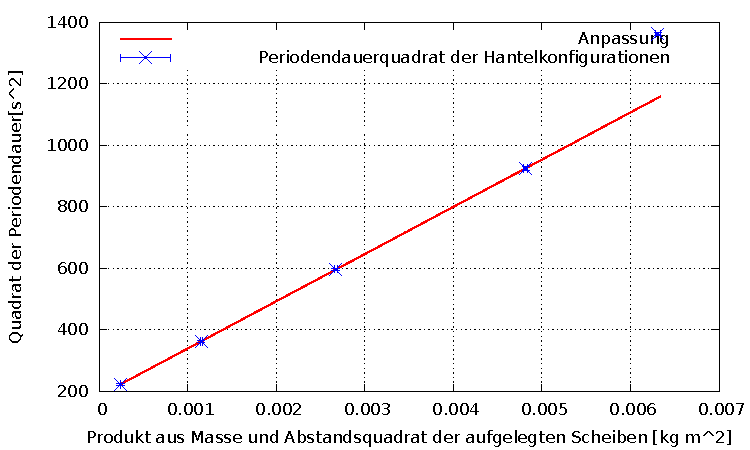
\includegraphics[width=0.7\linewidth]{auswertung/hantel/HantelF}
	\caption{Dargestellt werden die Messung mit Anpassung der Schwingungsdauern der Hantel mit aufgelegten Scheiben in verschiedenen Abständen zur Rotationsachse. Die Einheiten der Achsen sind so gewählt, dass die Messpunkte nach dem Steinerschen Satz linear sind.  }
	\label{fig:hantel}
\end{figure}

Der Steinersche Satz sagt einen linearen Zusammenhang für \cref{fig:hantel} vorher, daher wurde eine Anpassung des Typs $T^2(2m_2 a^2)=b (2m a^2)+c$ gewählt, da der letzte Messpunkt deutlich Abseits einer gedachten Grade durch die anderen Messpunkte lag, wurde hier von einem groben Fehler ausgegangen und er wurde bei der Anpassung ausgelassen.
Man erhält nach der Anpassung\footnote{Die Anpassung wurde durch "Gnuplot" mit dem Levenberg–Marquardt Algorithmus vorgenommen.  } und unter Berücksichtigung des geringen Freiheitsgrades (2) die Werte:
 $ b               = \SI{1.5346 \pm 0.004 e+005}{\second \squared \per \kilogram \per \metre \squared} $ und $c               = \SI{186.587\pm 1.1}   {\second \squared}$. Aus der Steigung $b$ und Gleichung \ref{eq:hantelta} folgt durch Koeffzientenvergleich $D^*=\SI{8.19+-0.02e-5}{\kilogram \metre \squared \per \second \squared }$ Da jedoch der letzte Punkt so stark abweicht nehmen wir eine Unsicherheit von $\Delta D^*= \SI{\pm 2e-6}{\kilogram \metre \squared \per \second \squared }$ an.


%t_p





Die Schwingungsdauer der Hantel ohne Scheiben $T_0$  betrug \SI{13.01 \pm 0.03}{s}. Es folgt mit Gleichung \ref{eq:hantelJ} für das Trägheitsmoment des Hantelstabes $J_1 = \SI{1.40+-0.04e-3}{\kilogram \metre \squared}$.



\begin{align}
	J=\frac{T^2 D^*}{4 \pi^2} \pm \frac{T^2 D^*}{4 \pi^2} \sqrt{
	\left(\frac{2 \Delta T}{T} \right)^2 + 	\left(\frac{\Delta D^*}{D^*} \right)^2 }
\label{eq:hantelJ}
\end{align}




Aus dem Parameter $c$ und der Gleichung \ref{eq:hantelta} und $a=0$  folgt für das Trägheitsmoment der Hantelscheiben mit Schwerpunkt auf der Rotationsachse die Gleichung \ref{eq:hantelJ2} und $J_2=\SI{5.1+-0.4e-5 }{\kilogram \metre \squared}$.


\begin{align}
		T^2&= \frac{4 \pi^2}{D^*}(J_1+2J_2+2m_2 a^2)
	\label{eq:hantelta}\\
J_2&=\frac{c D^*}{8 \pi ^2}-\frac{J_1}{2} \pm \sqrt{\left( \frac{c D^*}{8 \pi}\right) ^2\left( \left( \frac{\Delta c}{c}\right) ^2+  \left( \frac{\Delta D^*}{D^*}\right) ^2\right) + \left(\frac{J_1}{2}\right)^2 }\label{eq:hantelJ2}
\end{align}
\begin{align}
	J_{allg.}=\int r_{\perp}^2 \textrm{d}m
	\label{eq:Jallg}
\end{align}

Zum Vergleich wurden die theoretisch vorhergesagten Trägheitsmomente nach Gleichung \ref{eq:Jallg} bestimmt und in Tabelle \ref{tab:vglJ} mit den experimentell bestimmten zum Vergleich aufgeführt. 

\begin{table}[h!]
	\caption{Vergleich der experimentellen Trägheitsmomente mit den theoretisch berechneten}
	\begin{tabular}{|c|c|c|}
		\hline 
		Objekt &Theoretischer Wert	& Experimenteller Wert  \\ 
		\hline 
		Hantelstange $J_1$ &$\SI{1.324\pm 0.004 e-3}{}$	& $\SI{1.40\pm 0.04e-3}{}$ \\ 
		\hline 
		Scheibe $J_2$&  $\SI{5.76\pm 0.07e-5}{}$	&$\SI{5.1 \pm 0.5  e-04}{}$ \\ 
		\hline 
	\end{tabular} 
	\label{tab:vglJ}
\end{table}








\subsection{Diskussion}

%vgl mit lit wert am ehesten $\alpha$ Eisen $G=\SI{8.4 e9}{kg \per \metre \second \squared}$ abweichungen groß nicht aufgeführte legierung
Im Vergleich mit den Literaturwerten erscheint eine Stahllegierung wahrscheinlich. So besitzt zum Beispiel "CrV-Federstahl" oder "V2A-Stahl" ein Schubmodul\footnote{entnommen: Gerthsen Physik, Vogel 1977} $G=\SI{8.000 e10}{kg \per  \second \squared \metre}$.
Genauso Wahrscheinlich sind jedoch auch andere Stahllegierungen, da die Eigenschaften von den genauen Anteilen der Legierungsbestandteilen steuerbar sind und das gewünschte Schubmodul mit verschiedenen Zusätzen erreicht werden kann.\\
An den Werten in \cref{tab:vglJ}, dass der theoretische Wert für das Trägheitsmoment liegen jeweils in der $2 \sigma$-Umgebung des experimentell bestimmten Wertes und stellen somit keinen Widerspruch dar. Die weiteren berechneten Werte lassen sich nicht einordnen, da es sich um Materialkonstanten handelt und die Materialien nicht bekannt sind. Bei einer Weiterführung der Versuchsreihe wäre die Pendeldauer der Hantel für das größte $a$ zu wiederholen um zu überprüfen ob es sich wie angenommen um einen Fehler handelt oder ob die Abweichung reproduzierbar ist. Sollte eine höhere Genauigkeit erforderlich sein, sollte insbesondere $J_1$ genauer bestimmt werden, da dieser Wert für weitere Rechnungen benötigt wird. Eine höhere Genauigkeit von $D^*$, welches auch Grundlage weiterer Berechnungen ist, ist nur durch allgemeine Techniken wie mehr Abstände vermessen oder über viele Perioden mehrfach messen möglich und somit deutlich aufwendiger. 
%Tabbel Werte vgl Theorie exp....















%19

\section{Schlussfolgerung}
Im ersten Teil der Auswertung wurde der Eleatizitätsmodul $E$ bestimmt. Beim Vergleich von den Experimentell bestimmten Werten mit Literaturwerten fiel auf das die Vermutung das es sich bei der Messingfarbenden Runden Stange um Messing handelte vermutlich falsch ist, da die Werte für den Elastizitätsmodul 
























Das Torsionspendel eignete sich um den Schubmodul( $G =\SI{7.87+-0.09e10}{kg \per \second \squared  \metre}$) des verwendeten Drahtes bei bekanntem Trägheitsmoment zu bestimmen und durch diese Materialeigenschaft Rückschlüsse auf das verwendete Material (Stahllegierung) zu ziehen. Da der Schubmodul jedoch von dem Fertigungsprozess und den Beimengungen abhängt, ist dies nur als Richtwert zu verstehen. Bei bekanntem Schubmodul $G$ und den Abmessungen des Drahtes bzw. dem Direktionsmodul $D^*=\SI{8.2+-0.2e-5}{\kilogram \metre \squared \per \second \squared }$  lässt sich aus der Schwingungsdauer das jeweilige Trägheitsmoment berechnen.  Die gemessenen  Trägheitsmoment  sind \cref{tab:vglJ} zu entnehmen.











% --- Anhang einbinden
\IfFileExists{tex/20_Anhang.tex}{
	\clearpage
	\appendix
	\section{Anhang}
	\label{sec:anhang}
	

\subsection{Verwendete Gleichungen}\label{VGuD}
%und Definition der Variablen


%Zusammenhang zwischen Kreisfrequenz $\omega$ und Schwingungsdauer $T$:

%\begin{align}
%	T=\frac{2 \pi}{\omega} \pm \Delta t
%	\label{eq:T}
%\end{align} 


%Alle anderen Unsicherheiten sind gemäß Kapitel \ref{sec:einzeln} so klein, dass sie zu vernachlässigen sind. Es sei $\Delta t={ 0,006} {s}$.\\
%\frac{2 \pi}{\omega^2} \cdot\Delta \omega  \label{eq:T}


%Standardunsicherheit der Rechteckverteilung u für die Intervallbreite a:
	%\begin{align}
	%	u=\frac{a}{2\sqrt{3}}\label{eq:SR}
	%\end{align} 



}{}

% --- Literaturverzeichnis mit BibLaTeX
%\ifthenelse{\boolean{showBibliography}}{
%	\clearpage
%	\printbibliography
%}{}

\end{document}

